\chapter{Modely dielektrické odezvy amorfních materiálů}

Výběr vhodného disperzního modelu je pro správné vyhodnocení experimentálních dat klíčový. Hlavní požadavek, který klademe na zvolený model dielektrické odezvy, je ten, že musí dobře popisovat optické charakteristiky sytému, jako odrazivost, propustnost a~elipsometrické veličiny. Toho je možné dosáhnout tím, že parametrizujeme přímo komplexní index lomu případně komplexní dielektrickou funkci. Příklad takového jednoduchého modelu je například Cauchyho formule. Přestože takové modely mnohdy dosahují velmi dobrých výsledků při fitování experimentálních dat, neposkytují žádné informace o vnitřní struktuře měřené látky. Tato práce se proto bude zabývat modely, které poskytují informace i o~vnitřním uspořádáni materiálu, hlavně o parametrech elektronové struktury.

Z teorie dielektrické odezvy vyplývá několik podmínek, které musí každý vhodný model splňovat. První podmínkou jsou Kramers--Kronigovi relace, které spojují reálnou a~ima\-gi\-nární část dielektrické funkce  
\begin{equation}
\epsilon_\mathrm{r}(\omega) = 1 + \frac{1}{\pi} \mathcal{P} \int \frac{\epsilon_\mathrm{i}(\xi)}{\xi - \omega} \mathrm{d}\xi \mathrm{,}
\label{KKint}
\end{equation}
kde $\omega$ je úhlová frekvence a~$\epsilon_\mathrm{r}, \epsilon_\mathrm{i}$ jsou reálná a~imaginární část dielektrické funkce a~$\mathcal{P}$ značí Cauchyho hlavní hodnotu. 

Druhá podmínka, kterou musí lineární dielektrické odezvy splňovat, je časová symetrie
\begin{equation}
\epsilon(\omega) =\epsilon^* (-\omega) \mathrm{,}
\label{casovasymetrie}
\end{equation}
symbol $^*$ značí komplexní sdružení.

Třetí podmínka pro model dielektrické odezvy je takzvané f-sumační pravidlo
\begin{equation}
\int_0^\infty \epsilon_\mathrm{i} (\omega) \omega \mathrm{d} \omega = \frac{\pi}{2} \omega_\mathrm{p}^2 = \frac{\pi}{2} \frac{e^2 n_\mathrm{e}}{ \epsilon_0 m_\mathrm{e}} \mathrm{,}
\end{equation}
kde $\omega_\mathrm{p}$ je plazmová frekvence, $n_\mathrm{e}$ je koncentrace elektronů, $e$ je elementární náboj, $m_\mathrm{e}$ je hmotnost elektronu a~$\epsilon_0$ je permitivita vakua. F-sumační pravidlo je důsledek kombinace Kramers-Kronigova integrálu s předpokladem pro chování dielektrické odezvy pro $\omega \rightarrow \infty$ jako pro klasický tlumený oscilátor a~spojuje hustotu náboje s~dielektrickou funkcí. Klasické f-sumační pravidlo můžeme chápat jako integrální formu Thomas--Reiche--Kuhnova (TRK) sumačního pravidlo z kvantové mechaniky, pokud ho aplikujeme na interakci světla s pevnou látkou.  

Klasické sumační pravidlo bylo dále v \cite{sumrule} zobecněno pomocí TKR sumačního pravidla, aby zahrnovalo jak elektrony, tak atomová jádra do následujícího tvaru
\begin{equation}
\int_0^\infty \mathcal{F} \mathrm{d}E = n_e + \sum_n \frac{Z_n^2 m_\mathrm{e}} {m_n} n_n = U n_\mathrm{e} \mathrm{.} %FIXME
\end{equation}
Sumace je prováděna přes všechny typy jader v materiálu. Symboly $Z_n, m_n, n_n$ značí po řadě protonové číslo, hmotnost jádra a~koncentraci jader. $E$ je energie fotonu. Faktor $U$ je pro většinu materiálů velmi podobný: $U \approx 1.00027$ \cite{sumrule}.

Pro parametrizaci dielektrické funkce je praktické zavést funkci $F(E)$
\begin{equation}
F(E) = \epsilon_\mathrm{i}(E) E = \frac{\mathcal{F}(E)}{M}\mathrm{,}
\end{equation}  
kde $M$ je konstanta
\begin{equation} 
M = \frac{8 \pi \epsilon_0 m_\mathrm{e}}{(e h)^2} = 4,61706\times10^{26} \mathrm{eV}^{-2}\mathrm{m}^3 \mathrm{.}
\end{equation}

Funkci $F(E)$ nazýváme funkce síly přechodu a~slouží jako výchozí bod při parametrizaci optických konstant v pevných látkách. Jedná se o spojitou analogii síly oscilátoru.

\section{Parametrizace funkce dielektrické odezvy}
Dielektrická funkce může být rozdělena na více příspěvků, které reprezentují jednotlivé typy přechodů $t$. Celková dielektrická funkce je suma přes dielektrické funkce jednotlivých částí a~vakua \cite{sumrule}
\begin{equation}
\epsilon(E) = 1 + \sum_t \epsilon_t(E) \text{.}
\label{suma1}
\end{equation}

Dříve zavedenou funkci síly přechodu $F(E)$ můžeme také rozdělit na parciální funkce síly přechodu pro jednotlivé příspěvky $t$
\begin{equation}
F(E) = \sum_t F_t(E) \text{.}
\end{equation}
%Je praktické jednotlivé příspěvky $F_t$ normalizovat na $F_t^0$ aby platilo
%\begin{equation}
%\int_0^\infty F_t^0(E)\mathrm{d}E = 1
%\end{equation}
Integrováním přes $F_t(E)$ získáme 
\begin{equation}
\label{definiceceelkovesily}
\sum_t \int_0^\infty F_t(E)\mathrm{d}E = \sum_t N_t = N \text{,}
\end{equation}
$N_t$ jsou integrální síly přechodů pro jednotlivé příspěvky a~$N$ je celková integrální síla přechodu, nebo jen jednoduše celková síla přechodu.  

Dále můžeme zavést takzvanou normalizovanou dielektrickou funkci $\epsilon_t^0$ pro jednotlivé příspěvky. Platí 
\begin{equation}
\epsilon_t(E) = N_t \epsilon_t^0  \text{.}
\end{equation}

Pak můžeme přepsat vztah (\ref{suma1}) jako
\begin{equation}
\epsilon (E) = 1 + \sum_t N_t \epsilon_t^0(E) \text{.}
\end{equation}




\section{Jednotlivé příspěvky k dielektrické funkci}
Jelikož se v této práci zabýváme zkoumáním DLC vrstev, omezíme se pouze na příspěvky, z nichž se skládá dielektrická funkce právě v DLC vrstvách. Jedná se o přechody valenčních elektronů do vodivostních pásů a~vyšších excitovaných stavů, o excitaci jaderných elektronů a~o fononovou absorpci. 

\subsection{Mezipásové přechody mezi valenčním a~vodivostním pásem}
Absorpce světla v amorfních materiálech je způsobena přechodem elektronu z výchozího stavu $j$ s energií $S$ do konečného stavu $k$ s energií $S + E$. Imaginární část dielektrické funkce je spočítána jako suma příspěvků všech možných přechodů

\begin{equation}
\label{basicDOS}
\epsilon_\mathrm{i} (E) = 
\left(\frac{eh}{m_\mathrm{e}E} \right)^2 \frac{1}{4 \pi \epsilon_0 \mathrm{B}_0} \sum_{j,k} | p_{j \rightarrow k} |^2
\int_{-\infty}^\infty f_\mathrm{e}(S) \mathcal{N}_j(S) f_\mathrm{h}(S+E) \mathcal{N}_k(S + E)\mathrm{d}S \text{,}
\end{equation}
kde $E$, $h$ a~$\mathrm{B}_0$ jsou energie fotonu, Planckova konstanta a~určitá část Brillouinovy zóny odpovídajícího krystalického materiálu. Funkce $\mathcal{N}_j(S)$ a~$\mathcal{N}_k(S)$ značí rozdělení energií hustoty stavů (DOS) v $j$ a~$k$ pásu. Koncentrace $j$ elektronů, tj. počet $j$ elektronů na~jednotku objemu je definován jako
\begin{equation}
\mathrm{N}_j = \int_{-\infty}^\infty \mathcal{N}_j(S)\mathrm{d}S \text{.}
\end{equation}
Výše uvedené přechody jsou možné jen tehdy, pokud jsou $j$ stavy zaplněné a~$k$ stavy nejsou. To je v integrálu zahrnuto pomocí Fermi-Diracova rozdělení pro elektrony, $f_\mathrm{e}$, a~díry, $f_\mathrm{h}$. Pravděpodobnost přechodu je dána čtvercem velikosti maticového elementu operátoru hybnosti $|p_{j \rightarrow k}|^2$. Je vytknuta před integrál, protože předpokládáme, že je v amorfním materiálu konstantní pro všechny přechody mezi konkrétním $j$ a~$k$ pásem. Rovnice (\ref{basicDOS}) může zahrnovat jednak mezipásové přechody i přechody uvnitř pásu. DOS funkce $\mathcal{N}_j(S)$ a~$\mathcal{N}_k(S)$ mohou zahrnovat rozšířené i~lokalizované stavy. Pokud je valenční pás plně zaplněn a~vodivostní pás je zcela prázdný, můžeme Fermi-Diracovo rozdělení vynechat a~integrál ve vztahu (\ref{basicDOS}) poté definuje takzvanou funkci sdružené hustoty stavů (JDOS) $\mathcal{J}_{j \rightarrow k}(E)$ odpovídající $j \rightarrow k$ přechodům
\begin{equation}
\mathcal{J}_{j \rightarrow k}(E) = \int_{-\infty}^\infty \mathcal{N}_j(S) \mathcal{N}_k(S + E)\mathrm{d}S \text{.}
\end{equation}
Vztah (\ref{basicDOS}) nicméně definuje pouze imaginární část dielektrické funkce a~pouze pro kladné $E$. Celkovou komplexní dielektrickou funkci můžeme získat pomocí antisymetrie imaginární části (\ref{casovasymetrie}) a~Kramers-Kronigových relací (\ref{KKint})
\begin{equation}
\label{basicDLC2}
\epsilon_i (E) = 
\left(\frac{eh}{m_\mathrm{e}E} \right)^2 \frac{\mathrm{sgn}(E)}{4 \pi \epsilon_0 \mathrm{B}_0} \sum_{j,k} | p_{j \rightarrow k} |^2
\int_{-\infty}^\infty f_\mathrm{e}(S) \mathcal{N}_j(S) f_\mathrm{h}(S+|E|) \mathcal{N}_k(S + |E|)\mathrm{d}S \text{,}
\end{equation}

\begin{equation}
\epsilon_\mathrm{r}(E) = 
1 + \frac{1}{\pi} \mathcal{P} \int_{-\infty}^\infty \frac{\xi \epsilon_\mathrm{i}(\xi)}{\xi^2 - E^2} \mathrm{d}\xi = 
1 + \frac{2}{\pi} \mathcal{P} \int_0^\infty \frac{\xi \epsilon_\mathrm{i}(\xi)}{\xi^2 - E^2} \mathrm{d}\xi 
\text{.}
\end{equation}


Vhodný model nyní můžeme sestrojit parametrizací DOS funkcí, příkladem takového modelu je PDOS model \cite{franta2007}. Model zjednodušuje rovnici (\ref{basicDLC2}) zavedením schodové Fermi-Diracovy funkce (což je splněno, pokud pásy leží v dostatečné vzdálenosti od Fermiho energie) a~zavedením funkce $\mathfrak{N}$, která v sobě zahrnuje konstanty před integrálem 
\begin{equation}
\label{epsilonDOS}
\epsilon_\mathrm{i}(E) = \frac{\mathrm{sgn}(E)}{E^2} \sum_{j} \int_{-\infty}^{E_\mathrm{F} = 0} \mathfrak{N}_j(S) \mathfrak{N}_{j^*}(S + |E|)\mathrm{d}S \text{,}
\end{equation}
kde
\begin{equation}
\label{unormN}
\mathfrak{N}_j(S) = \frac{eh | p_{j \rightarrow j^*} |}{2 m_\mathrm{e} \sqrt{\pi \epsilon_0 \mathrm{B}_0}} \mathcal{N}_j(S) \text{.}
\end{equation}
Index $j$, zde jde přes všechny typy elektronových stavů (v DLC vrstvách se například jedná o $\sigma$ a~$\pi$ elektrony), $j$ značí valenční elektrony $j^*$ vodivostní. $\mathfrak{N}_j(S)$ není nicméně, na rozdíl od $\mathcal{N}_j$, normován na koncentraci $j$ elektronů $\mathrm{N}_j$. Je proto výhodné zavést normovací parametr $Q_j$
\begin{equation}
\int_{-\infty}^\infty \mathfrak{N}_j(S) \mathrm{d}S = 
\mathrm{N}_j \frac{eh | p_{j \rightarrow j^*} |}{2 m_\mathrm{e} \sqrt{\pi \epsilon_0 \mathrm{B}_0}} \equiv
Q_j \text{,}
\end{equation}
kde parametr $Q_j$ je přímo úměrný koncentraci $j$ elektronů a~je jeden z parametrů PDOS modelu. Další dva parametry potřebné pro popis $j \rightarrow j^*$ přechodů jsou minimální energie, neboli šířka zakázaného pásu, $E_\mathrm{g}$ a~maximální energie přechodů $E_\mathrm{h}$. 

Díky podobnosti s distribucí hustoty stavů v krystalech v blízkosti extrému energie v pásu můžeme modelovat $\mathfrak{N}_j(S)$ a~$\mathfrak{N}_{j^*}$ pomocí odmocnin

\begin{equation}
\label{N1}
 \mathfrak{N}_j(S) = 
\frac{
		32Q_j 
		\sqrt{-S-\frac{E_{\mathrm{g}j}}{2}}
		\sqrt{\frac{E_{\mathrm{h}j}}{2}+S}
	}{
		\pi (E_{\mathrm{h}j} - E_{\mathrm{g}j})^2
	}
\text{,}
\end{equation}

\begin{equation}
\label{N2}
\mathfrak{N}_{j^*}(S) = 
\frac{
		32Q_j 
		\sqrt{S-\frac{E_{\mathrm{g}j}}{2}}
		\sqrt{\frac{E_{\mathrm{h}j}}{2}-S}
	}{
		\pi (E_{\mathrm{h}j} - E_{\mathrm{g}j})^2
	}
\text{,}
\end{equation}
Dosazení rovnic (\ref{N1}) a~(\ref{N2}) do (\ref{epsilonDOS}) získáme
\begin{equation}
\epsilon_\mathrm{i} = \frac{1}{E^2} \sum_j \left(\frac{32Q_j}{\pi (E_{\mathrm{h}j} - E_{\mathrm{g}j})^2}\right)^2 e_j(E) \text{,}
\end{equation}
kde $e_j(E)$ značí eliptický integrál, který musí být spočítán numericky
\begin{equation}
e(E) = \int_{S_\mathrm{min}}^{S_\mathrm{max}}
\sqrt{\left(-S - \frac{E_\mathrm{g}}{2}\right)\left(\frac{E_\mathrm{h}}{2} + S\right)}
\sqrt{\left(E + S - \frac{E_\mathrm{g}}{2}\right)\left(\frac{E_\mathrm{h}}{2} -E - S\right)}
\mathrm{d}S\,\,\Pi_{E_{\mathrm{g}},E_{\mathrm{h}}}(|E|)\text{.}
\end{equation}
kde funkce $\Pi_{E_\mathrm{min},E_\mathrm{max}}(|E|)$ je definována následovně
\begin{equation}
\Pi_{E_\mathrm{min},E_\mathrm{max}}(|E|) = 
	\left\{\begin{array}{l c l} 
	1 & : & E_\mathrm{min} < E < E_\mathrm{max} \\
	0 & : & \text{jinak.} \end{array} \right.
\end{equation}
Integrační meze eliptického integrálu jsou 
\begin{equation}
\begin{array}{l c r}
S_\mathrm{min} = \max\left(-\frac{E_\mathrm{h}}{2}, \frac{E_\mathrm{g}}{2} -E\right) &
\text{a} &
S_\mathrm{max} = \min\left(-\frac{E_\mathrm{g}}{2}, \frac{E_\mathrm{h}}{2} -E\right) \\
\end{array}
\end{equation}



Právě nutnost numerických kalkulací (jednak eliptického integrálu a~jednak Kramers--Kronigových relací) je mírnou nevýhodou PDOS modelu. Je proto výhodné parametrizovat přímo JDOS funkci tak, abychom se vyhnuli numerickým výpočtům. Toto řeší tzv. PJDOS model, který je kompromisem mezi rychlostí výpočtu a~kvalitou parametrizace odrážející skutečný stav pásové struktury. 

Podobně jako jsme zavedli nenormalizovanou DOS funkce $\mathfrak{N}_j$ (\ref{unormN}), zavedeme nyní nenormalizovanou PJDOS funkci $\mathfrak{J}_{j \rightarrow j^*}$
\begin{equation}
\left(\frac{eh}{m_\mathrm{e}} \right)^2 \frac{| p_{j \rightarrow j^*} |^2}{4 \pi \epsilon_0 \mathrm{B}_0} \mathcal{J}_{j \rightarrow j^*}(E)
= \mathfrak{J}_{j \rightarrow j^*}(E) \text{.}
\end{equation}
Tuto funkci můžeme stejně jako DOS funkce $\mathfrak{N}{j}$ a~$\mathfrak{N}{j}^*$ normovat na parametr elektronové hustoty $Q_j$
\begin{equation}
\int_0^\infty \mathfrak{J}_{j \rightarrow j^*}(E)\mathrm{d}E = Q_j^2 \text{.}
\end{equation}
Nyní je potřeba potřeba vhodně parametrizovat funkci $\mathfrak{J}_{j \rightarrow j^*}$, snažíme se zachovat co nejvytší podobu s DOS parametrizací (s eliptickým integrálem). Toto vede na následující tvar
\begin{equation}
\mathfrak{J}_{j \rightarrow j^*} \propto (E - E_{\mathrm{g}j})^2 (E - E_{\mathrm{h}j})^2 \text{.}
\end{equation} 
Výsledná podoba dielektrické funkce je tedy
\begin{equation}
\label{PJDOS1}
\epsilon_{\mathrm{i},j \rightarrow j^*}(E) = 
\frac{30Q_j (E - E_{\mathrm{g}j})^2 (E - E_{\mathrm{h}j})^2 }{(E_{\mathrm{h}j} - E_{\mathrm{g}j})^5 E^2 } 
\Pi_{E_{\mathrm{g}j},E_{\mathrm{h}j}}(|E|)
\text{,}
\end{equation}

V \cite{sumrule2} je model PJDOS rozšířen dále o parametry $E_\mathrm{c}$ a~$B_\mathrm{c}$ zahrnující rozšíření pásové struktury a~její nesymetrii vzhledem k Fermiho energii????? FIXME, výsledná normovaná dielektrická funkce má tvar

\begin{equation}
\label{valencvod}
\epsilon_{\mathrm{i},j \rightarrow j^*}^0 = 
\mathrm{sgn}(E) 
\frac	{(|E|- E_{\mathrm{g}j})^2(E_{\mathrm{h}j} - |E|)^2}
	{ C E^2 [(|E| - E_{\mathrm{c},j})^2 + B_{\mathrm{c},j}^2]} 
\Pi_{E_{\mathrm{g}j},E_{\mathrm{h}j}}(|E|) \, \mathrm{,}
\end{equation}
kde $C$ je normalizační konstanta.

\subsection{Excitace valenčních elektronů do vyšších excitovaných elektro-nových stavů}
Přestože jsou energie excitací do vyšších excitovaných pásů většinou již mimo oblast energií běžných optických metod a~jejich příspěvek se tedy v imaginární části dielektrické funkce neprojeví vůbec a~v reálné jen mírně, nemůžeme je zanedbat, protože hrají významnou roli v sumačním pravidle, kde integrujeme přes celou dielektrickou funkci, potřebujeme tedy alespoň odhad tvaru dielektrické funkce i pro vyšší energie. 
Můžeme je popsat dvouparametrickým modelem popsaným v \cite{sumrule}.
\begin{equation}
\label{vyssiexcitace}
\epsilon_{\mathrm{i}, j \rightarrow \xi}^0(E) = \frac{3 E_\xi(|E| - E_\xi)^2}{E^5} \Pi_{E_xi, \infty}(|E|) \text{,}
\end{equation}
kde $E_\xi$ je minimální energie přechodu do vyššího excitovaného stavu
\begin{equation}
E_\xi = \frac{E_{\mathrm{g},j}}{2} + E_\mathrm{x}
\end{equation}
Reálná část parciální dielektrické funkce má potom následující tvar
\begin{equation}
\epsilon_{\mathrm{r}, j \rightarrow \xi}(E) = 
\frac{3E_\xi}{\pi E^2}
\left[
	a(E) \ln\left|1-\frac{E}{E_\xi}\right|
	+ b(E) \ln\left|1 + \frac{E}{E_\xi}\right|
	- \frac{2}{3E_\xi} - \frac{2E_\xi}{E^2}
\right] \text{,}
\end{equation}
kde
\begin{equation}
\begin{array}{c c}
a(E) = -\frac{(E_\xi - E)^2}{E^3} &
b(E) = \frac{(E_\xi + E)^2}{E^3} \text{.}\\
\end{array}
\end{equation}


\subsection{Excitace jaderných elektronů}
U atomů, které mají kromě valenční elektronů i vnitřní slupky s ,,jadernými elektrony'' musíme zahrnout i vliv jejich excitací. Stejně jako u excitací valenčních elektronů do vyšších excitovaných stavů se projeví na dielektrické funkci v měřené oblasti pouze minimálně, nicméně opět tento příspěvek nemůžeme vynechat kvůli sumačnímu pravidlu. Normalizovaná dielektrická funkce pro excitace jaderných elektronů je modelována jednoduchým jednoparametrickým vzorcem \cite{sumrule2}
\begin{equation}
\label{jaderneel}
\epsilon_{\mathrm{i},\zeta}(E) = \frac{E_\zeta}{E^3} \Pi_{E_\zeta,\infty}(|E|) \text{,}
\end{equation}
\begin{equation}
\epsilon_{\mathrm{r},\zeta}(E) = \frac{1}{\pi E^3}\left[ E_\zeta \ln\left| \frac{E_\zeta + E}{E_\zeta - E} - 2E\right| \right] \text{,}
\end{equation}
kde $E_\zeta = E_i + E_\mathrm{g}/2$, $i$ indexuje všechny typy jaderných elektronů v atomu (K, L, ...). 

\subsection{Fononová absorpce}
V infračervené oblasti se ve spektrech DLC vrstev vyskytuje velké množství absorpčních píků, způsobených absorpcí na vibračních stavech C a~C--H skupin. Jednotlivé píky je možno modelovat jako Gausovské funkce v imaginární části dielektrické funkce \cite{franta2007}:

\begin{equation}
\label{gaus}
\epsilon^0_{\mathrm{i},p} = \frac{1}{\sqrt{2 \pi} B_p E_p} \left[ \exp\left(-\frac{(E-E_p)^2}{2B_p^2}\right) - \exp\left(-\frac{(E+E_p)^2}{2B_p^2}\right) \right] \text{.}
\end{equation}
V reálné části tomu odpovídá tvar:
\begin{equation}
\epsilon^0_{\mathrm{r},p} = \frac{\sqrt{2}}{\pi B_p E_p} \left[ \mathrm{D}\left(\frac{E+E_p}{\sqrt{2}B_p}\right) -\mathrm{D}\left(\frac{E-E_p}{\sqrt{2}B_p}\right) \right] \text{,}
\end{equation}
kde $\mathrm{D}(x)$ značí Dawsonův integrál, definovaný jako:
\begin{equation}
\mathrm{D}(x) = \exp(-x^2)\int_0^x \exp(t^2) \mathrm{d}t
\end{equation}
V infračervené spektroskopii je nicméně zvykem používat k popisování píků vlnočty místo energií. Z toho důvodu jsou parametry $E_p$ a~$B_p$ nahrazeny parametry $\tilde{\nu}_p$ a~$\beta_p$:
\begin{equation}
E_p = h c \tidle{\nu}_p \text{,}
\end{equation}
\begin{equation}
B_p = \frac{h c \beta_p}{2 \sqrt{2 \ln 2}} \text{,}
\end{equation}
kde $c$ je rychlost světla. 




\section{Aplikace na DLC vrstvy (model PJDOS-DLC)}
V této práci byly DLC vzorky modelovány jako multivrstvy: systém vrstva -- přechodová vrstva -- substrát -- zadní vrstva (obrázek \ref{layerscheme}). Pro modelování dielektrické funkce vrstvy byl použit model PJDOS-DLC, pro modelování přechodové vrstvy byl použit model PJDOS, pro křemíkový substrát byl použit model PJDOS c-Si a~pro modelování zadní vrstvy byly využity tabulkové hodnoty SiO$_2$.

\begin{figure}[h]
\centering
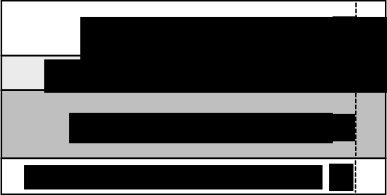
\includegraphics[width=12cm]{grafika/layerscheme.pdf}
\caption{Schéma multivrstevnatého systému s použitými modely pro jednotlivé části, $d_i$ jsou tloušťky jednotlivých vrstev}
\label{layerscheme}
\end{figure} 

\subsection{Vrstva}
Pro modelování dielektrické funkce DLC vrstvy byl použit model PJDOS-DLC \cite{franta2007}. Ten zahrnuje jednak přechody mezi valenčním a~vodivostním pásem (\ref{valencvod}) pro $\sigma$ a~$\pi$ elektrony, pak také excitace do vyšších excitovaných stavů nad vodivostním pásem (\ref{vyssiexcitace}), absorpci na vibračních stavech v infračervené oblasti (\ref{gaus}) a~excitaci jaderných elektronů (\ref{jaderneel}). Zjednodušené schéma elektronové struktury DLC vrstvy je na obrázku \ref{DLCDOS}.

\begin{figure}[h]
\centering
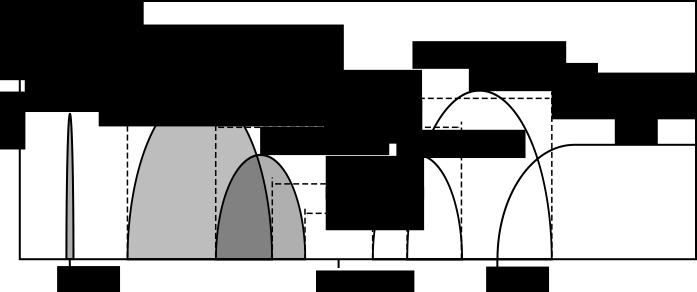
\includegraphics[width=15cm]{grafika/DLCDOS.pdf}
\caption{Schéma hustoty stavů DLC vrstvy}
\label{DLCDOS}
\end{figure} 

DLC vrstvu uvažujeme jako systém tří komponent: vodíkových jader, uhlíkových jader a~elektronů. Celkovou sílu přechodu $N$ můžeme proto rozepsat jako:
\begin{equation}
N = \int_0^\infty \epsilon_\mathrm{i}(E) E \mathrm{d}E = N_\mathrm{e} + N_\mathrm{C} + N_\mathrm{H} \text{,}
\end{equation} 
kde $N_\mathrm{e}$, $N_\mathrm{C}$ a~$N_\mathrm{H}$ jsou částečné síly přechodu pro elektrony, uhlíková jádra a~vodíková jádra. Pro atomy uhlíku můžeme navíc rozlišit sílu přechodu pro sp2 a~sp3 vázaný uhlík $N_\mathrm{C_{sp3}}$, $N_\mathrm{C_{sp2}}$
\begin{equation}
N_\mathrm{C} = N_\mathrm{C_{sp3}} + N_\mathrm{C_{sp2}} \text{.}
\end{equation} 
Jednotlivé síly přechodů závisí pouze na složení a~hustotě systému:
\begin{equation}
N_\mathrm{e} = [Z_\mathrm{C}f_\mathrm{C} + Z_\mathrm{H} f_\mathrm{H}] N_\mathrm{a} = (6f_\mathrm{C} + f_\mathrm{H})N_\mathrm{a} \text{,}
\end{equation}
\begin{equation}
N_\mathrm{C} = Z^2_\mathrm{C} f_\mathrm{C} \frac{m_\mathrm{e}}{m_\mathrm{C}} N_\mathrm{a} \text{,}
\end{equation}
\begin{equation}
N_\mathrm{H} = Z^2_\mathrm{H} f_\mathrm{H} \frac{m_\mathrm{e}}{m_\mathrm{H}} N_\mathrm{a} \text{,}
\end{equation}
kde $N_\mathrm{a}$ značí atomovou koncentraci a~$f_\mathrm{H}$, $f_\mathrm{C}$ jsou relativní koncentrace vodíku a~uhlíku ($f_\mathrm{H} + f_\mathrm{C} = 1 $). $Z_\mathrm{C}$ a~$Z_\mathrm{H}$ značí atomové čísla uhlíku a~vodíku. $m_\mathrm{e}$, $m_\mathrm{C}$ a~$m_\mathrm{H}$ jsou hmotnost elektronu, hmotnost jádra uhlíku a~hmotnost jádra vodíku. 

Celkovou sílu přechodu $N$ také můžeme vyjádřit podle (\ref{definiceceelkovesily}) jako součet jednotlivých příspěvků $t$

\begin{equation}
N = N_\mathrm{v} + N_\mathrm{K} + \sum_i N_{\mathrm{p},j} \text{.}
\end{equation}

$N_\mathrm{v}$ zde značí sílu kombinovanou sílu přechodu pro valenční elektrony jednak do vodivostního pásu a~jednak do excitovaných stavů nad vodivostním pásem, $N_\mathrm{K}$ značí sílu přechodu pro K jaderné elektrony a $\sum_i N_{\mathrm{p},j}$ značí kombinovanou sílu přechodu pro všechny vibrační stavy mřížky $j$. Sílu přechodu $N_\mathrm{v}$ můžeme rozložit na části pro $\sigma$ a~$\pi$ elektrony $N_\sigma$, $N_\pi$ podle jejich poměru (na jeden sp2 atom uhlíku připadá jeden $\pi$ elektron a~tři $\sigma$ elektrony, na sp3 vázaný uhlík čtyři $\sigma$ elektrony a~na vodík pouze jeden $\sigma$  elektron)
\begin{equation}
N_\pi = N_\mathrm{v} \frac{f_\mathrm{C_{sp2}}}{4f_\mathrm{C} + f_\mathrm{H}}  \text{,}
\end{equation}
\begin{equation}
N_\sigma = N_\mathrm{v} \frac{4f_\mathrm{C_{sp3}} + 3f_\mathrm{C_{sp2}} + f_\mathrm{H}}{4f_\mathrm{C} + f_\mathrm{H}}  \text{.}
\end{equation}

$N_\sigma$ a~$N_\pi$ můžeme opět rozložit na části určující sílu přechodů mezi valenčním a~vodivostním pásem a~mezi valenčním pásem a~vyššími excitovanými stavy
\begin{equation}
\begin{array}{lr}
N_{\sigma \rightarrow \xi} = N_\mathrm{\sigma} \alpha_{\sigma\xi} \text{,} &
N_{\sigma \rightarrow \sigma^*} = N_\sigma - N_{\sigma \rightarrow \xi} \text{,} \\
\end{array}
\end{equation}
\begin{equation}
\begin{array}{lr}
N_{\pi \rightarrow \xi} = N_\mathrm{\pi} \alpha_{\pi\xi} \text{,} &
N_{\pi \rightarrow \pi^*} = N_\pi - N_{\pi \rightarrow \xi} \text{.} \\
\end{array}
\end{equation}

Dále je potřeba rozdělit sílu přechodu pro fononové absorpce $N_\mathrm{p}$ na síly přechodu jednotlivých píků
\begin{equation}
N_\mathrm{p} = \sum_j N_{\mathrm{p},j} \text{,}
\end{equation}
kde $j$ reprezentuje všechny možné vibrační stavy ve vrstvě. Navíc platí, že síly přechodu pro jednotlivé vibrační stavy jsou přímo úměrné částečným silám přechodu pro vodíková, případně uhlíková jádra můžeme tedy zavést relativní síly přechodů pro jednotlivé vibrační stavy $\alpha_j$
\begin{equation}
N_{\mathrm{p},j} = 
	\left\{\begin{array}{l c l} 
	\alpha_j N_\mathrm{H} & : & \text{pro j vibrační mód vodíkových skupin} \\
	\alpha_j N_\mathrm{C} & : & \text{pro j vibrační mód uhlíkových skupin.}\end{array} \right.
\end{equation}
Podobně platí, že síla přechodu pro excitaci jaderných elektronů, je přímo úměrná síle přechodu uhlíkových jader, je proto výhodné zavést relativní sílu přechodu pro excitaci jaderných elektronů $\alpha_\mathrm{K}$
\begin{equation}
N_\mathrm{K} =  \alpha_\mathrm{K} N_\mathrm{C}
\end{equation}

Celkově tedy v modelu PJDOS-DLC vystupuje 16 + 3$j$ parametrů. Tři parametry související se složením materiálu $N_\mathrm{a}$, $f_\mathrm{C_{sp3}}$ a~$f_\mathrm{H}$. Dva parametry pro modelování jaderných elekronů $\alpha_\mathrm{K}$ a~$E_\mathrm{K}$. Osm parametrů pro modelování přechodů mezi valenčním a~vodivostním pásem $\sigma$ a~$\pi$ elektronů $E_\mathrm{g\{\pi,\sigma\}}$, $E_\mathrm{h\{\pi,\sigma\}}$, $E_\mathrm{c\{\pi,\sigma\}}$ a~$B_\mathrm{c\{\pi,\sigma\}}$. Tři parametry pro přechody do vyšších energetických stavů $E_\mathrm{x}$, $\alpha_{\{\sigma,\pi\}\xi}$ a~tři parametry pro každý přítomný vibrační stav $\alpha_j$, $\nu_j$ a~$\beta_j$.

Přehledně všechny parametry shrnuje tabulka \ref{DLCparametry}.

\begin{table}
\centering
\begin{tabular}{l l}
\hline

$N_\mathrm{a}$ & atomová koncentrace \\
$f_\mathrm{C_{sp3}}$ & relativní koncentrace sp3 uhlíku \\
$f_\mathrm{H}$ & relativní koncentrace vodíku \\

$\alpha_\mathrm{K}$ & relativní síla přechodu pro K jaderné elekrony\\
$E_\mathrm{K}$ & vzdálenost středu pásu K elektronů od Fermiho energie\\

$E_\mathrm{g\{\pi,\sigma\}}$ & šířka zakázaného pásu \{$\pi$, $\sigma$\} elektronů\\
$E_\mathrm{h\{\pi,\sigma\}}$ & maximální energie přechodu \{$\pi$, $\sigma$\} elektronů\\
$E_\mathrm{c\{\pi,\sigma\}}$ & FIXME \{$\pi$, $\sigma$\} elektronů\\
$B_\mathrm{c\{\pi,\sigma\}}$ & FIXME \{$\pi$, $\sigma$\} elektronů\\

$E_\mathrm{x}$ & vzdálenost hrany pásu vyšších excitací od Fermiho energie\\
$\alpha_{\{\sigma,\pi\}\xi}$ & relativní síly přechodu \{$\sigma$,$\pi$\} elektronů do vyšších excitovaných stavů \\

$\alpha_j$ & relativní síla přechodu $j$-tého vibračního módu \\
$\nu_j$ & poloha $i$-tého vibračního módu\\
$\beta_j$ & pološířka $i$-tého vibračního módu\\
\hline

\end{tabular}
\label{DLCparametry}
\caption{Parametry modelu PJDOS-DLC}
\end{table}

\subsection{Přechodová vrstva}
Mezi DLC vrstvou a~krystalickým křemíkem se nachází mezivrstva, tlustá často i desítky nanometrů, vzniklá implantací vysokoenergetických iontů uhlíku do krystalického křemíku. Její optické konstanty jsou proto někde mezi krystalickým křemíkem a amorfním DLC. Pro parametrizaci přechodové vrstvy byl použit jednoduchý tříparametrický PJDOS model (\ref{PJDOS1}) reprezentující přechody mezi jedním valenčním a vodivostním pásem a s jedním gausovským píkem (\ref{gaus}) ve viditelné oblasti, který reprezentuje absorpci na defektních stavech??? (defect states)???

\subsection{Substrát}
Jako substrát byl u všech vzorků použit krystalický křemík (111) o tloušťce přibližně 0,36\,mm. Při modelování substrátu byly postupně vyzkoušeny tři metody. První verze použitých modelů využívaly tabulkové hodnoty dielektrických funkcí krystalického kře\-mí\-ku. Tento postup byl dostatečný pro viditelnou a~ultrafialovou oblast, kde je křemík neprůhledný a~kde na jeho optické vlastnosti nemají vliv případné příměsi. V infračervené oblasti se nicméně ukázaly jako problém příměsi kyslíku, které vzorek od vzorku mírně kolísaly a~způsobovaly odlišnou absorpci hlavně v oblasti pod 1100\,cm$^{-1}$. Druhým vyzkoušeným řešením bylo proto naměřit absorpci křemíkového substrátu před depozicí, nafitovat optické konstanty substrátu samostatně a~použít je následně při fitování vrstvy. Tato metoda se nicméně také neosvědčila, hlavně kvůli velké časové náročnosti a~také kvůli tomu, že koncentrace kyslíkových příměsí se mírně liší i v rámci jednoho vzorku.
Nakonec byl tedy substrát fitován zároveň s vrstvou. Bylo k tomu použit model PJDOS-cSi \cite{}, jako volný parametr byla zvolena pouze koncentrace kyslíkových příměsi $f_\mathrm{O}$ a~tloušťka křemíkového waferu $d_\mathrm{s}$ (která také mírně kolísala).  

\subsection{Zadní vrstva}
Ze zadní strany křemíkového substrátu se vlivem oxidace vytvoří tenká vrstva SiO$_2$, o tloušťce několik nanometrů. Toto nepředstavuje problém pro viditelnou a ultrafialovou oblast, kde je křemík neprůhledný, ale projevuje se to infračervené oblasti, zvýšenou absorpcí v oblasti pod 1100\,cm$^{-1}$, hlavně v místech, kde se vyskytují výrazné píky SiO$_2$ (okolo 1075\,cm$^{-1}$, 460\,cm$^{-1}$ a 800cm$^{-1}$). Tento vliv jen možno odstranit přidáním zadní vrstvy do modelu vícevrstevnatého systému s zafixovanými hodnotami optických konstant pro SiO$_2$ získaných z \cite{palik1985handbook}.

\cleardoublepage
